\chapter{Theoretical Background}

\section{Active Galactic Nuclei}

Active Galactic Nuclei (AGN) are among the brightest and most energetic objects in the known universe, with bolometric luminosities ranging from $10^{41}$ to $10^{48}\,\mathrm{erg\,s^{-1}}$, surpassing those of other galaxies by many orders of magnitude. AGN emit radiation across the entire electromagnetic spectrum, from radio waves to gamma rays. In the optical and ultraviolet bands, their spectrum is dominated by the "Big Blue Bump" which is attributed to thermal emission from a hot accretion disc surrounding a central supermassive black hole. AGN spectra also exhibit strong emission lines: broad lines (FWHM up to $25.000\,\mathrm{km\,s^{-1}}$) produced by fast-moving gas in the Broad-Line Region (BLR), and narrower lines from the more distant, slower gas in the Narrow-Line Region (NLR) \parencite{peterson1997introduction}.\\\\
AGNs can be broadly grouped into so called Seyfert galaxies, quasars and radio galaxies. Seyfert galaxies are further subdivided, based on the width of their optical emission lines and radio properties. Seyfert 1 Galaxies show broad emission lines, while Seyfert 2 Galaxies show only narrow emission lines, narrow-line Seyfert 1 galaxies (NLS1), low-ionization nuclear emission-line regions (LINERs), and BL Lac objects or blazars \parencite{antonucci1993unified,urry1995unified}.\\\\
Figure \ref{fig:agn_sed} shows the unification model of an AGN. 
As illustrated an AGN is powered by a supermassive black hole surrounded by several distinct regions. Closest to the black hole is the accretion disc, whose hot, optically thick gas emits the thermal “Big Blue Bump” in the optical/UV bands \parencite{peterson1997introduction}. Encircling the disc is the Broad-Line Region (BLR), a compact area of dense clouds orbiting at thousands of kilometres per second, which produces the broad emission lines. Outside the BLR lies the dusty torus, a toroidal structure of cooler gas and dust that can obscure the inner regions when viewed edge-on \parencite{antonucci1993unified}. Beyond the torus, the more extended Narrow-Line Region (NLR) emits narrower lines from slower gas at distances of hundreds of parsecs. In radio-loud AGN, powerful relativistic jets emerge perpendicular to the disc plane, accelerating particles to near-light speeds and generating strong radio emission \parencite{urry1995unified}.


\begin{figure}[!ht]
	\centering
	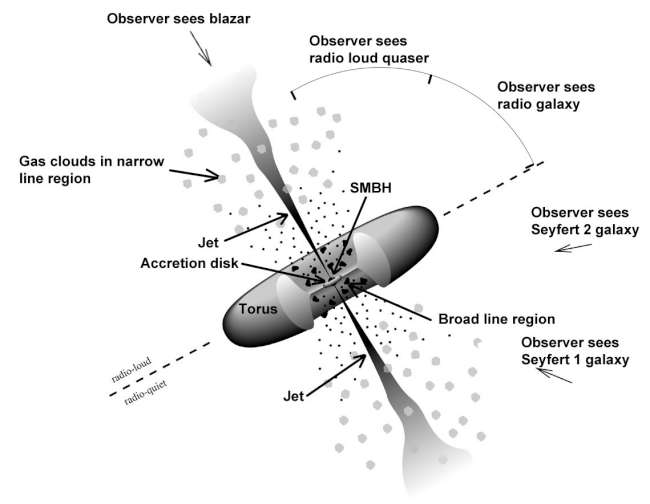
\includegraphics[width=\textwidth]{pictures/Chapter1/AGN_unified_model.jpg}
	\caption{Unification model of an AGN \parencite{fermi2025figure1}.}
	\label{fig:agn_sed}
\end{figure}



\section{Reverberation Mapping}



The main focus of this work was to perform a classic reverberation analysis of NGC 4593, with a focus on the broad line region (BLR) and its geometry around the central supermassive black hole (SMBH).\\\\
This type of analysis aims to measure the time lag $\tau$ between the variable continuum and the emission line response, in order to determine the spatial scale and structure of the BLR. By observing these variations over time and analyzing the delayed response of the broad lines, it is possible to learn more about the geometry and dynamics of the BLR and to estimate the mass of the SMBH.\\\\
Reverberation mapping (RM) is based on the strong correlation between a variable continuum emission $C(t)$ and the emission line flux $L(\nu, t)$ \parencite{horne2021space}. This correlation originates from the photoionization of gas clouds in the BLR by the central continuum source. As the continuum changes, the emission lines react in a similar way, but with a time delay $\tau$, because of the distance between the central source and the BLR. This delay corresponds to the time it takes for light to travel from the central source to the BLR.\\\\